\documentclass{deliverablereport}
\usepackage{pdfpages}

\deliverable{UI}{pari-python-lib1}
\deliverydate{10/02/2017}
\duedate{01/03/2016 (M6)}
\author{Luca De Feo, Vincent Delecroix, and Jeroen Demeyer}

\begin{document}
\enlargethispage{4ex}
\maketitle
\githubissuedescription
\tableofcontents\newpage


\section{Rationale}

The \Sage project includes many different subsystems, mostly written
in C/C++. For each subsystem, \Sage provides a low-level interface,
usually written in \Cython, through which the higher level components
access the subsystem. The mathematical community would immensely
benefit if the low-level interfaces were maintained outside of the
\Sage project, as separate \Python packages. Indeed such decoupling
would enable other \Python projects to build upon those externalized
interfaces, thus helping improve them, and share maintenance effort.

Of all the subsystems, the case of \Pari is of particular
interest. Since its inception, \Sage has had a low-level \Cython
interface to \Pari, which has evolved over time in a highly coupled
way. Around 2012, some \Sage developers forked this interface into a
project they called
\href{https://bitbucket.org/t3m/cypari/}{CyPari}. One of the primary
goals of the CyPari fork was to make independent \Python bindings to
\Pari for use in a project called
\href{https://bitbucket.org/t3m/snappy}{Snappy}. Over time, the CyPari
fork has diverged from the \Sage/\Pari interface, and has gotten
behind in terms of functionality.

The goal of this deliverable was to reconcile the fork by
externalizing the \Sage/\Pari interface into an independent package,
maintained by the \Sage community, which may ultimately replace CyPari
inside Snappy. 


\section{Work accomplished}

Completing this deliverable happened to be more difficult than
originally planned. The high level of coupling between \Sage internals
and the \Pari interface makes it very delicate to pull the latter out
of the \Sage codebase. Initially planned to be delivered in month 6,
it was only completed in month 16.

The process of making this deliverable possible led to a great amount
of refactoring inside the \Sage project. As summarized in
\href{http://trac.sagemath.org/ticket/20238}{Trac ticket 20238} (see
appendix), it required close to 50 \emph{tickets}, which fell in the
following categories:

\begin{itemize}
\tightlist
\item Moving \Sage's C signalling api to a separate \Python/\Cython
  package called
  \href{https://github.com/sagemath/cysignals}{cysignals}.
\item Decoupling \Sage's \Pari interface from the \emph{coercion
    model}.
\item Upgrading the \Pari interface to the latest upstream version
  (2.8.0).
\item Cleaning up the \Pari interface API, by removing unneeded object
  orientation and external dependencies.
\item Moving the \Pari interface to a separate \Python/\Cython package
  \href{https://github.com/sagemath/cysignals}{cysignals}, depending
  on cysignals.
\end{itemize}

The end results of this work are the packages
\href{https://github.com/sagemath/cysignals}{cysignals} and
\href{https://github.com/sagemath/cypari2}{CyPari2}, both installable
in a pure \Python environment via the standard tool
\texttt{pip}. Starting from version 7.6, installation via \texttt{pip}
will also be \Sage's default way of providing the \Pari interface.


\section{Aftermath}

The CyPari2 package is not ready to replace CyPari yet. The most
important missing functionality is Windows compatibility. A full
replacement to CyPari is the goal of
deliverable~\longdelivref{UI}{pari-python-lib2}.

Because of the high degree of coupling, and thanks to the availability
of a third party tool depending on it in Snappy, this deliverable
constitutes a highly valuable case study for future externalizations
of low-level interfaces in \Sage. Recently, the \Sage developer
community has increasingly paid attention to interoperability, as
highlighted by the many related discussions on the
\href{https://groups.google.com/forum/#!forum/sage-devel}{sage-devel}
mailing list.  We are confident that the experience gained in
developing this deliverable will be an accelerator for making \Sage a
more modular and interoperable software distribution.

\clearpage
\appendix
\section{Sage's Trac ticket \#20238}

\enlargethispage{1cm}

\url{http://trac.sagemath.org/ticket/20238}

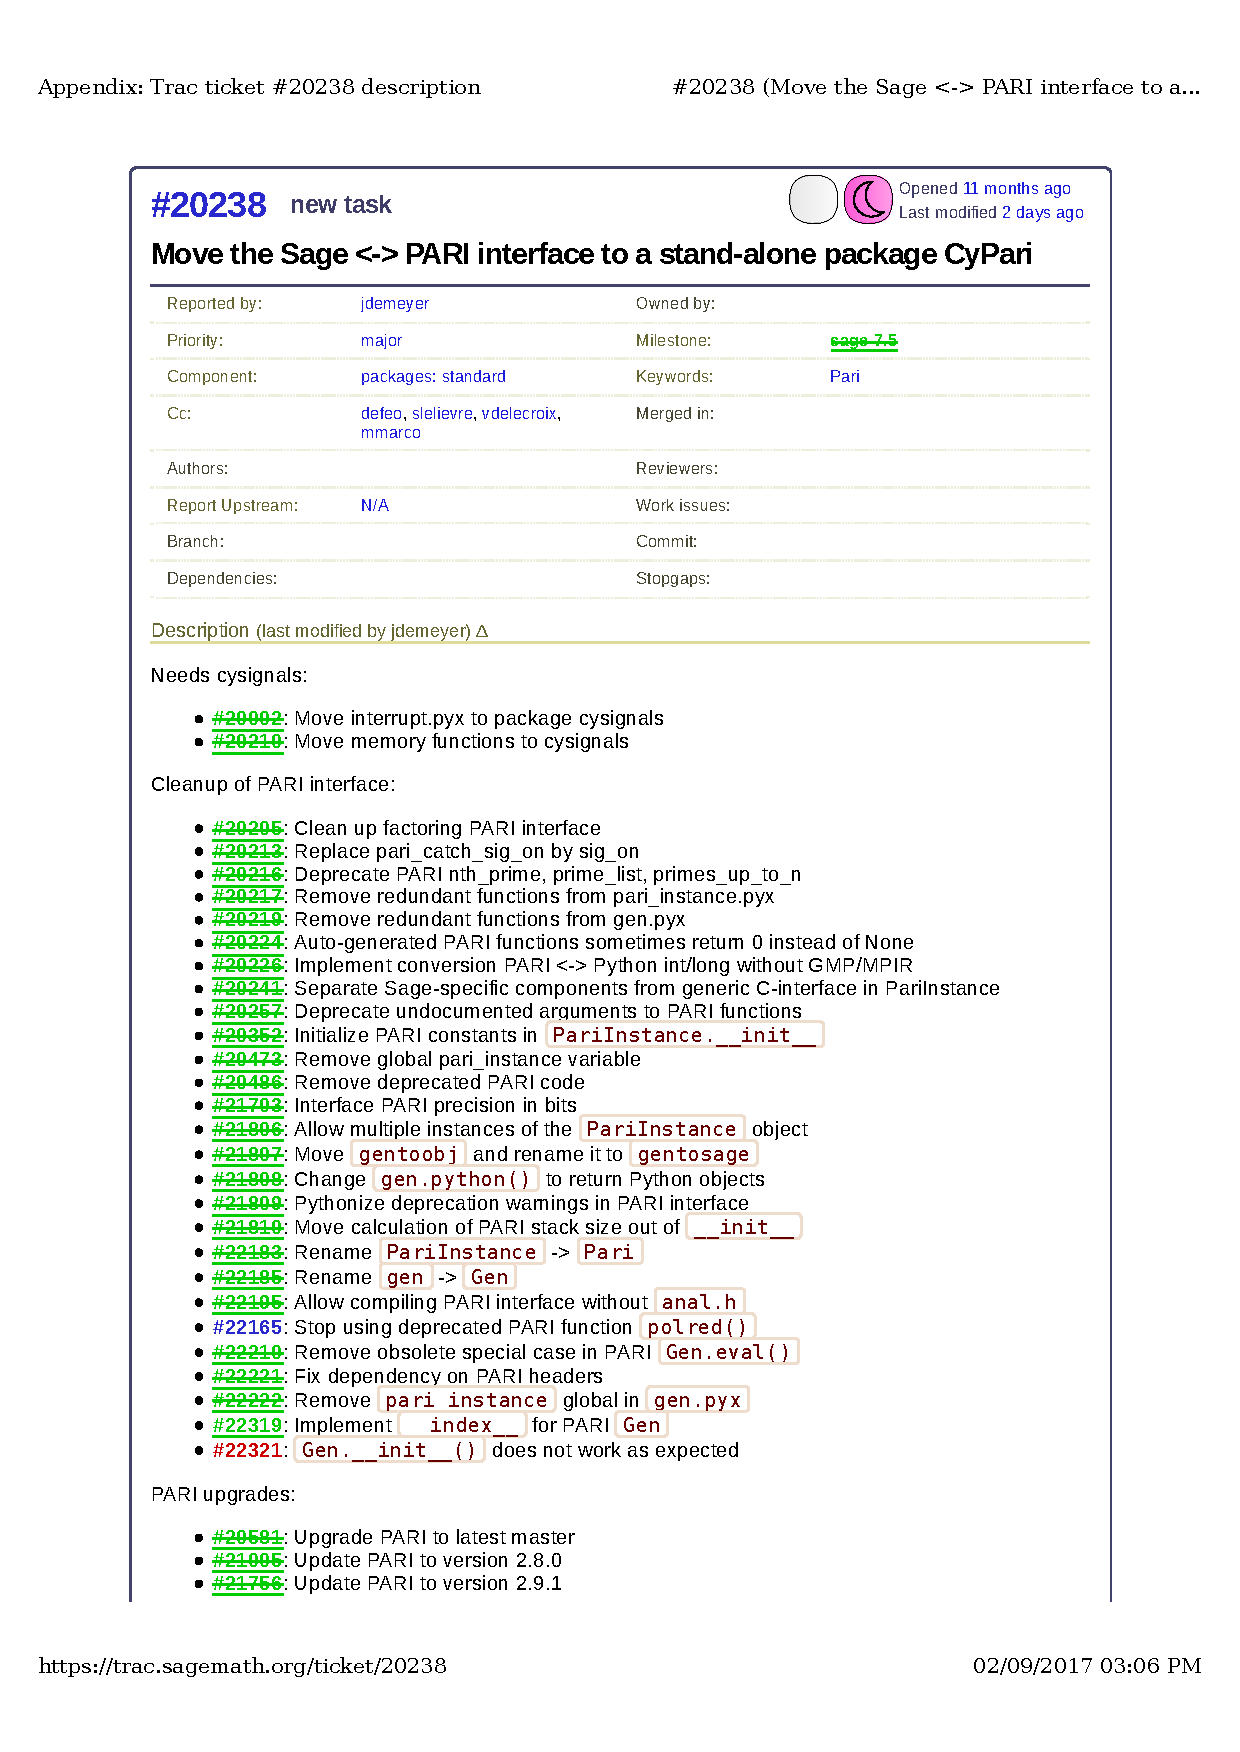
\includegraphics[clip, trim=2.2cm 2.5cm 2.2cm 2.5cm, width=1.00\textwidth]{ticket-20238}
\clearpage

\end{document}
